% Auto-generated by 08_export_results_to_manuscript.py.
% Include from main.tex with: % Auto-generated by 08_export_results_to_manuscript.py.
% Include from main.tex with: % Auto-generated by 08_export_results_to_manuscript.py.
% Include from main.tex with: % Auto-generated by 08_export_results_to_manuscript.py.
% Include from main.tex with: \input{generated/inputs.tex}

% ==== FIGURES ====
% \begin{figure}[h]
%   \centering
%   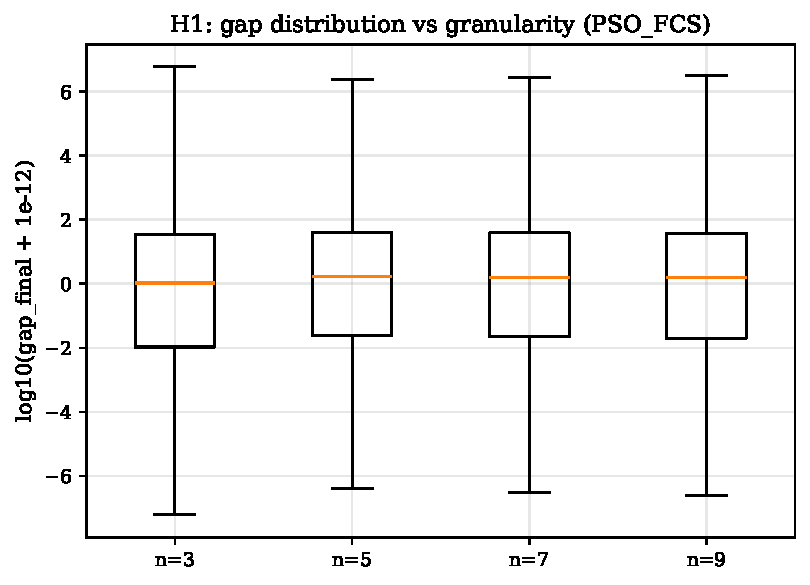
\includegraphics[width=0.85\linewidth]{figures/fig_boxplot_gap_by_n.pdf}
%   \caption{TODO caption for fig_boxplot_gap_by_n.}
%   \label{fig:fig_boxplot_gap_by_n}
% \end{figure}
% \begin{figure}[h]
%   \centering
%   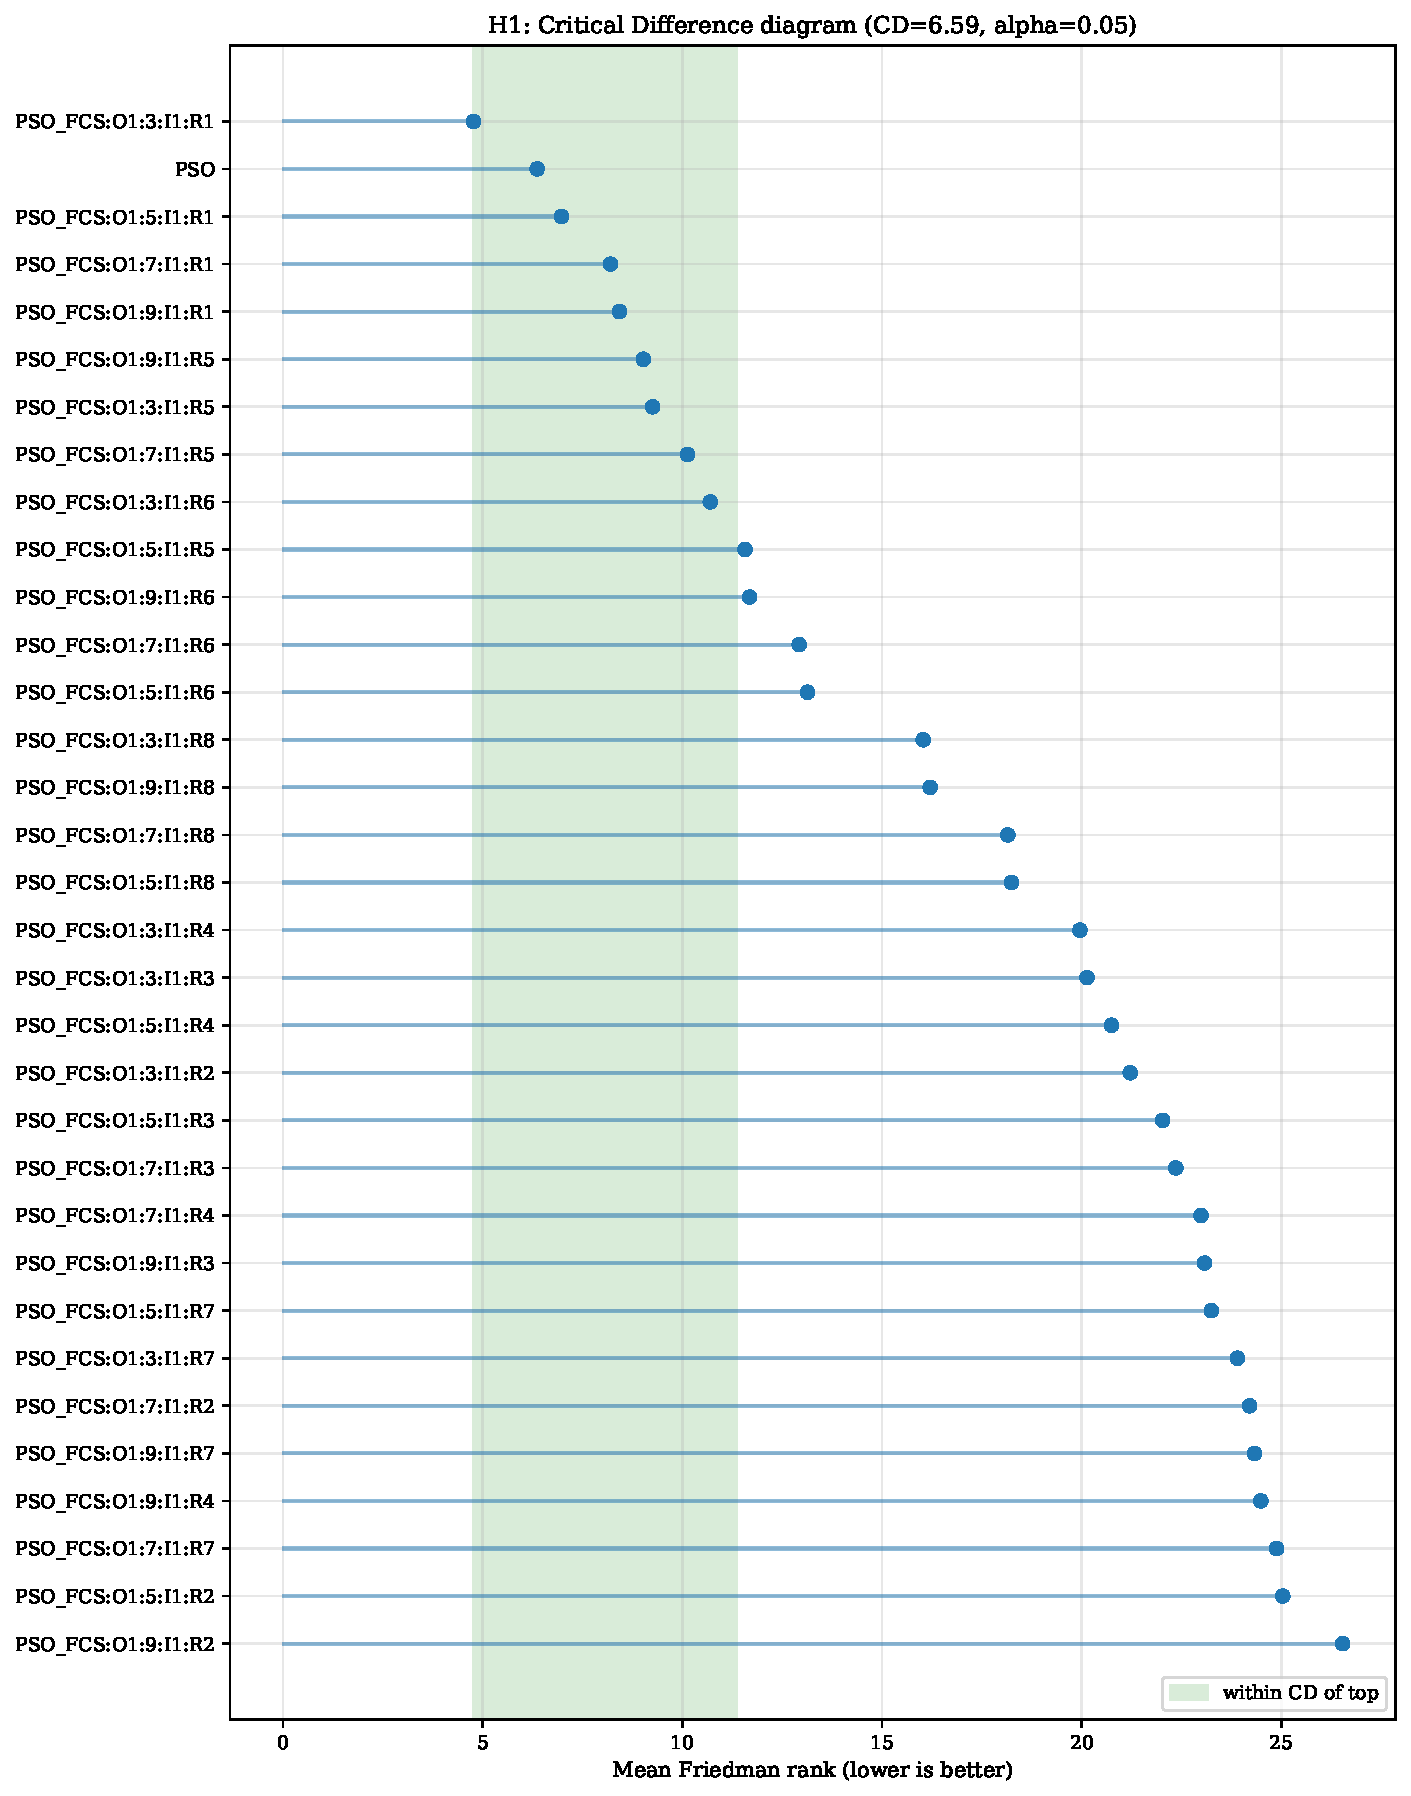
\includegraphics[width=0.85\linewidth]{figures/fig_cd_diagram_h1.pdf}
%   \caption{TODO caption for fig_cd_diagram_h1.}
%   \label{fig:fig_cd_diagram_h1}
% \end{figure}
% \begin{figure}[h]
%   \centering
%   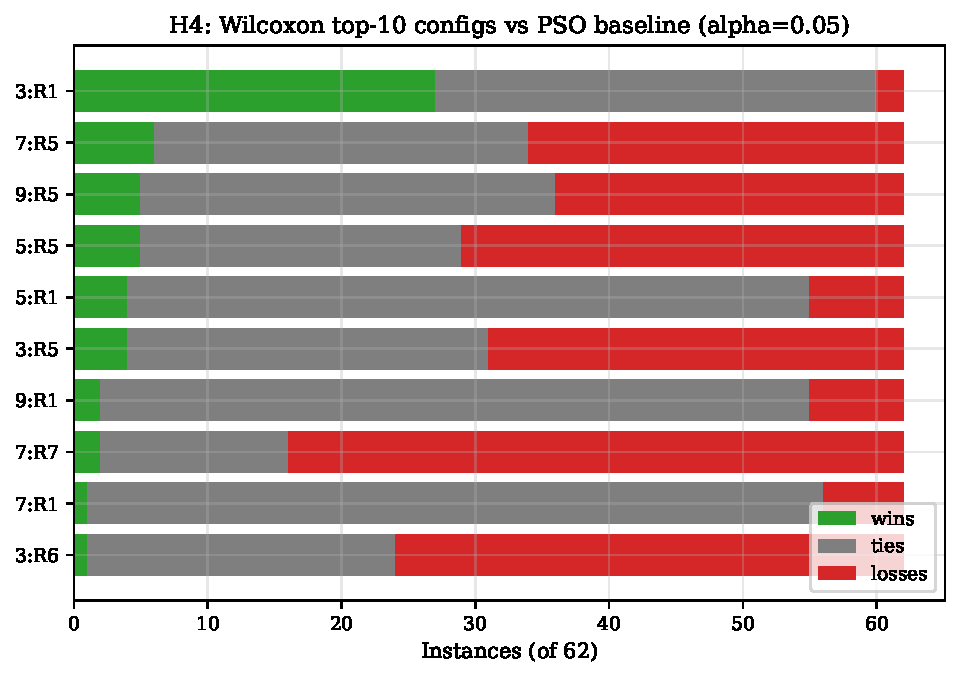
\includegraphics[width=0.85\linewidth]{figures/fig_h4_wilcoxon_bars.pdf}
%   \caption{TODO caption for fig_h4_wilcoxon_bars.}
%   \label{fig:fig_h4_wilcoxon_bars}
% \end{figure}
% \begin{figure}[h]
%   \centering
%   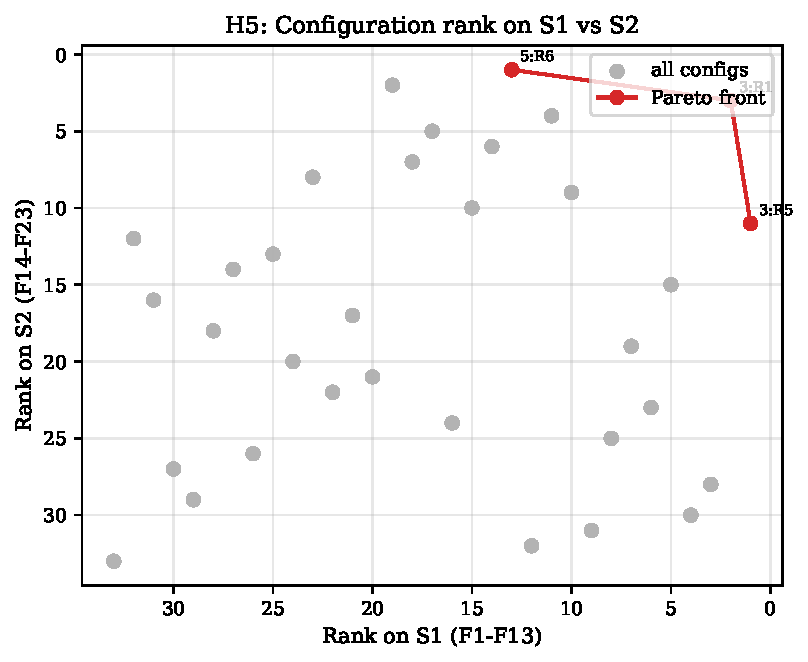
\includegraphics[width=0.85\linewidth]{figures/fig_pareto_s1_s2.pdf}
%   \caption{TODO caption for fig_pareto_s1_s2.}
%   \label{fig:fig_pareto_s1_s2}
% \end{figure}
% \begin{figure}[h]
%   \centering
%   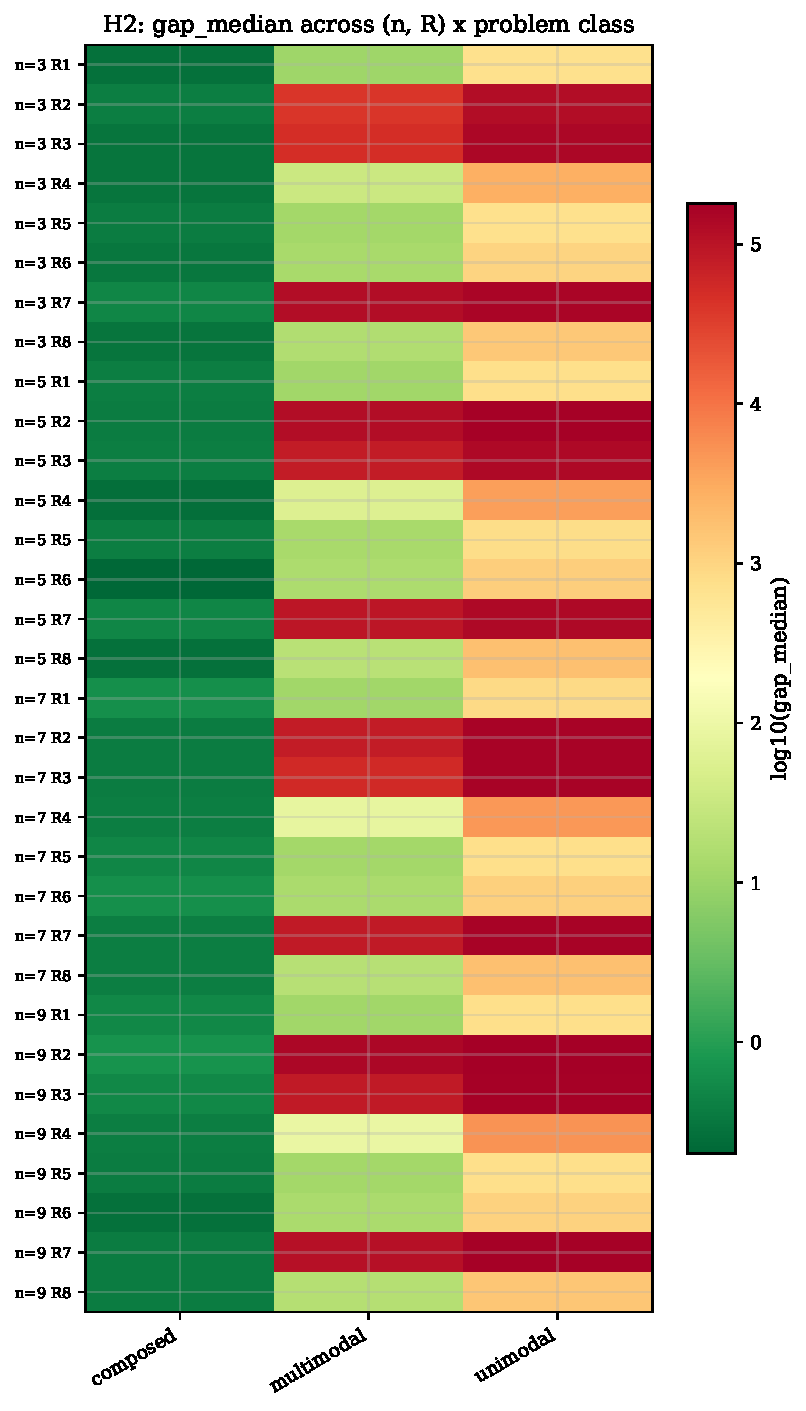
\includegraphics[width=0.85\linewidth]{figures/fig_rule_class_heatmap.pdf}
%   \caption{TODO caption for fig_rule_class_heatmap.}
%   \label{fig:fig_rule_class_heatmap}
% \end{figure}
% \begin{figure}[h]
%   \centering
%   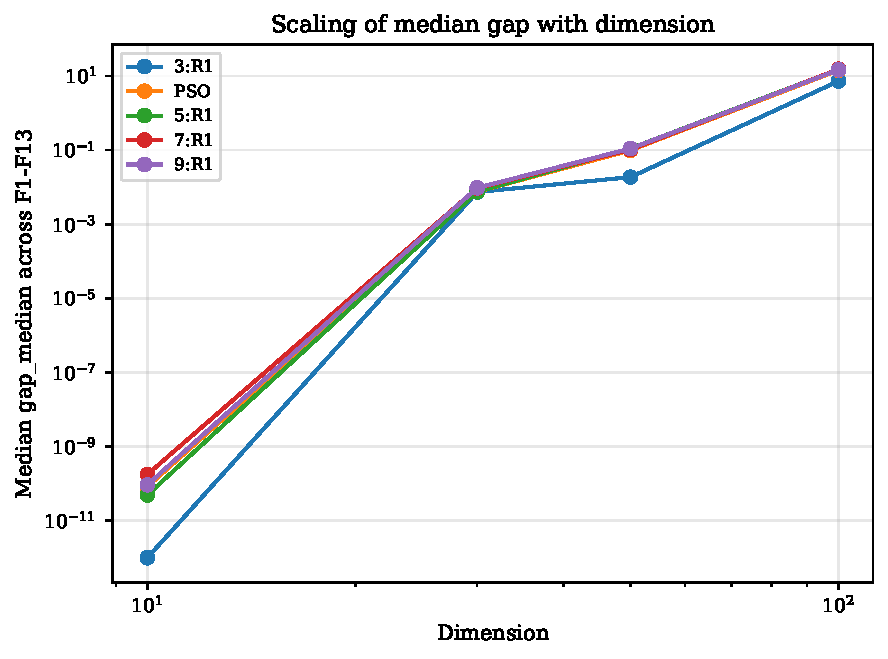
\includegraphics[width=0.85\linewidth]{figures/fig_scaling_curves.pdf}
%   \caption{TODO caption for fig_scaling_curves.}
%   \label{fig:fig_scaling_curves}
% \end{figure}
% \begin{figure}[h]
%   \centering
%   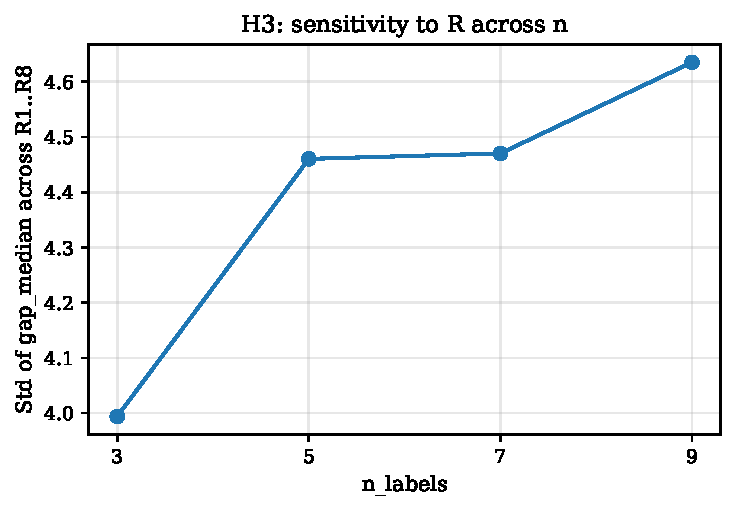
\includegraphics[width=0.85\linewidth]{figures/fig_std_R_vs_n.pdf}
%   \caption{TODO caption for fig_std_R_vs_n.}
%   \label{fig:fig_std_R_vs_n}
% \end{figure}

% ==== TABLES ====
% \input{tables/tab_h4_wilcoxon.tex}
% \input{tables/tab_hypothesis_summary.tex}
% \input{tables/tab_kendall_class.tex}
% \input{tables/tab_scaling_slopes.tex}
% \input{tables/tab_top_configs.tex}


% ==== FIGURES ====
% \begin{figure}[h]
%   \centering
%   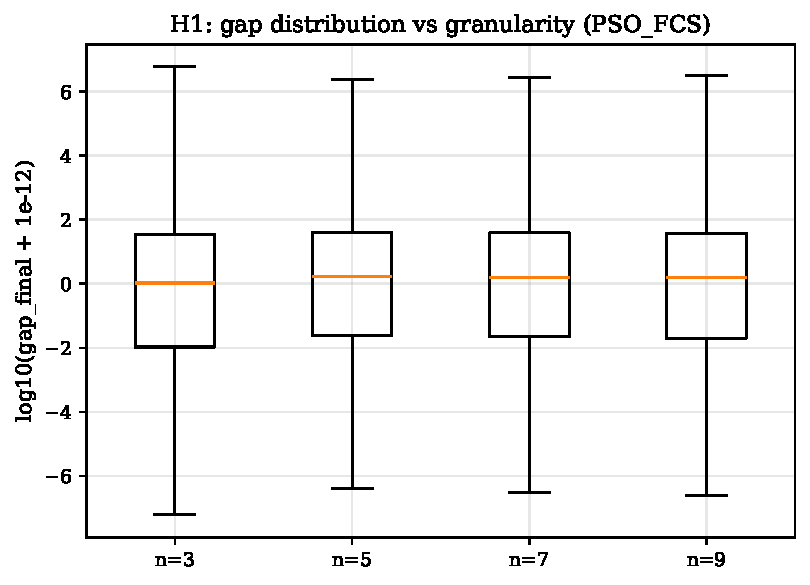
\includegraphics[width=0.85\linewidth]{figures/fig_boxplot_gap_by_n.pdf}
%   \caption{TODO caption for fig_boxplot_gap_by_n.}
%   \label{fig:fig_boxplot_gap_by_n}
% \end{figure}
% \begin{figure}[h]
%   \centering
%   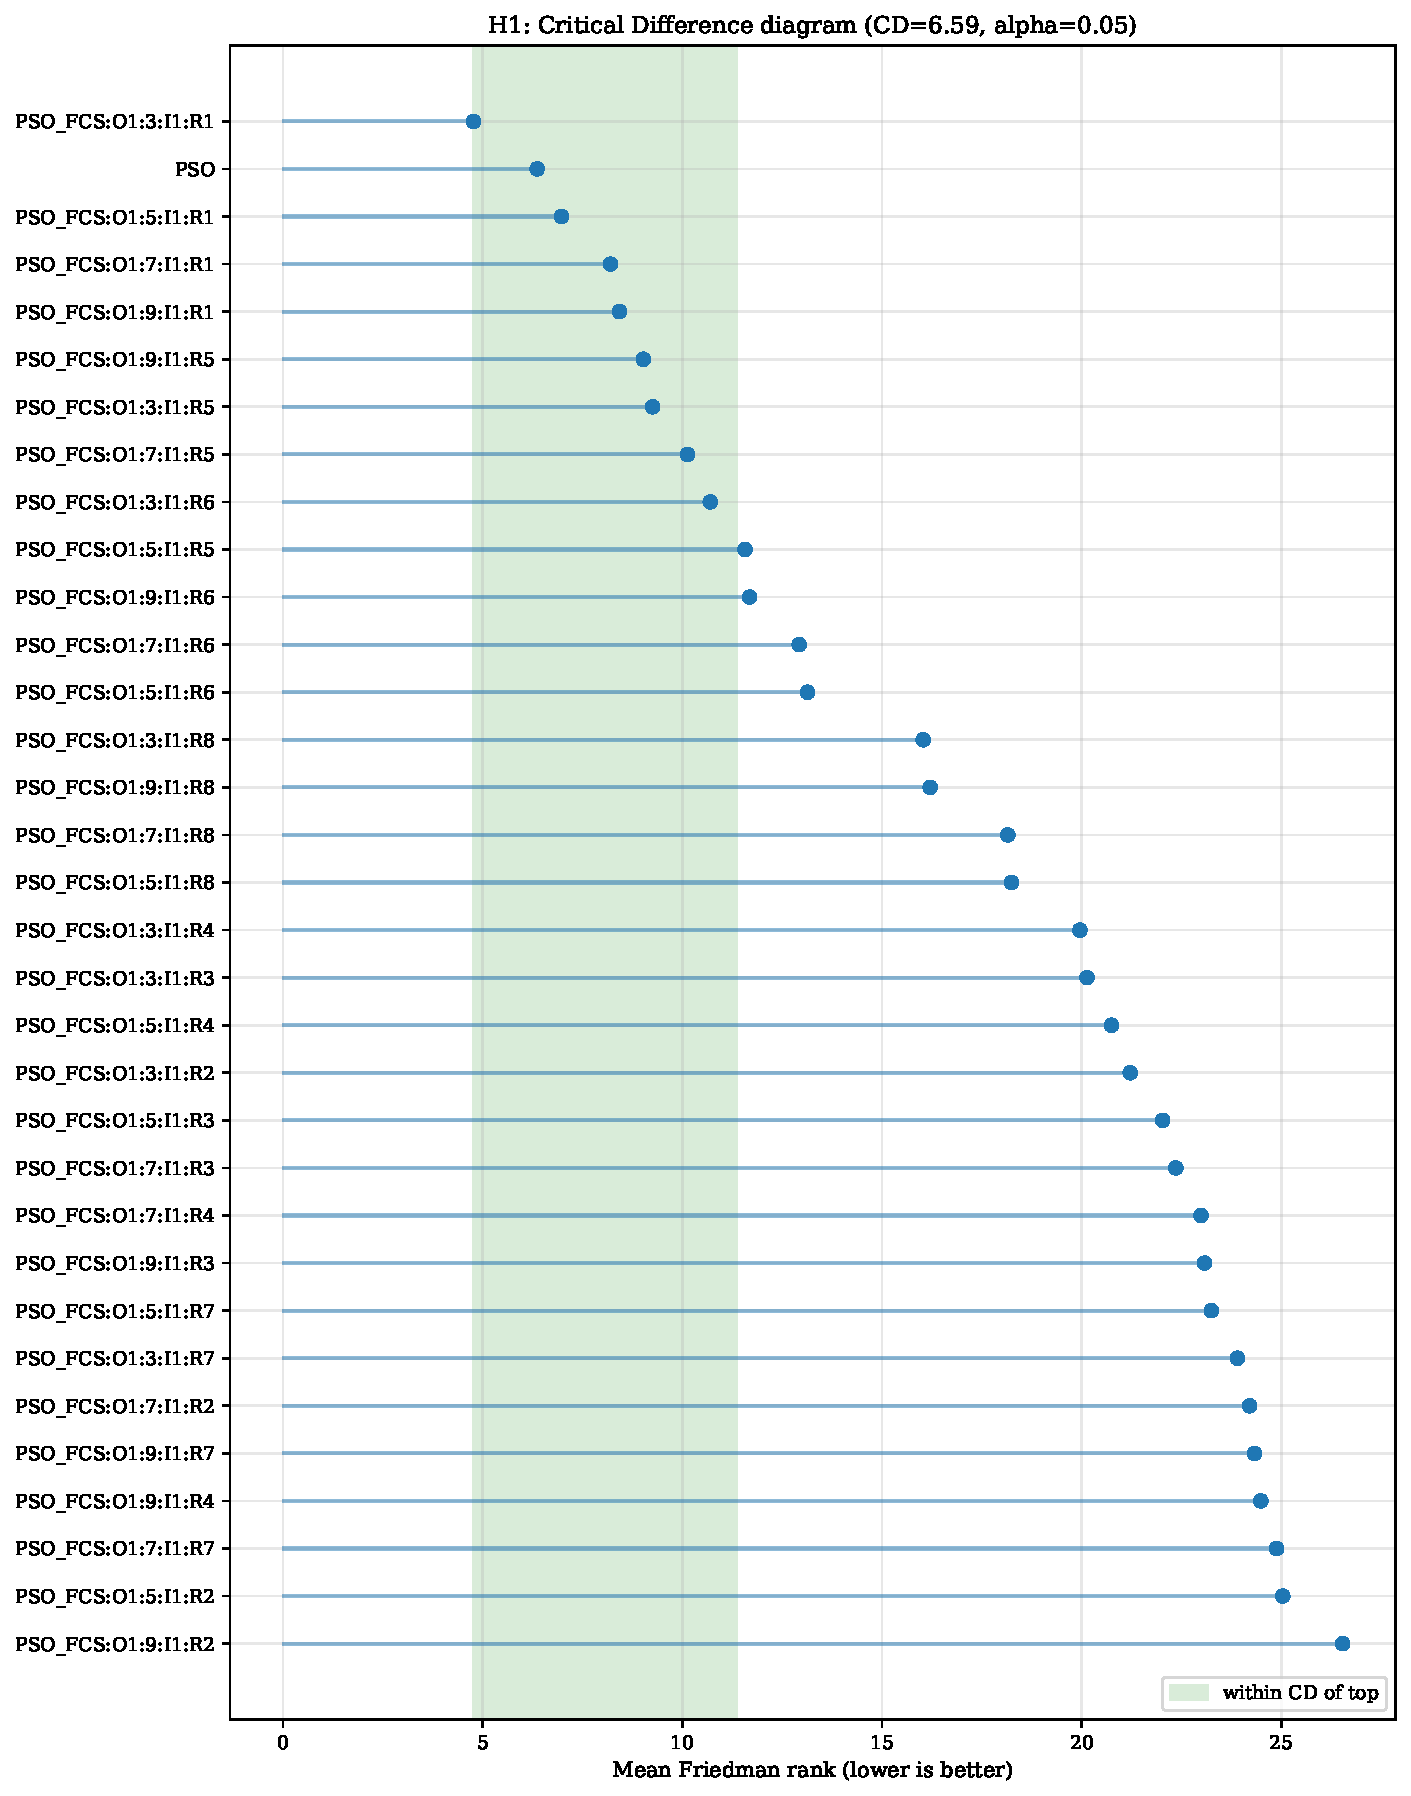
\includegraphics[width=0.85\linewidth]{figures/fig_cd_diagram_h1.pdf}
%   \caption{TODO caption for fig_cd_diagram_h1.}
%   \label{fig:fig_cd_diagram_h1}
% \end{figure}
% \begin{figure}[h]
%   \centering
%   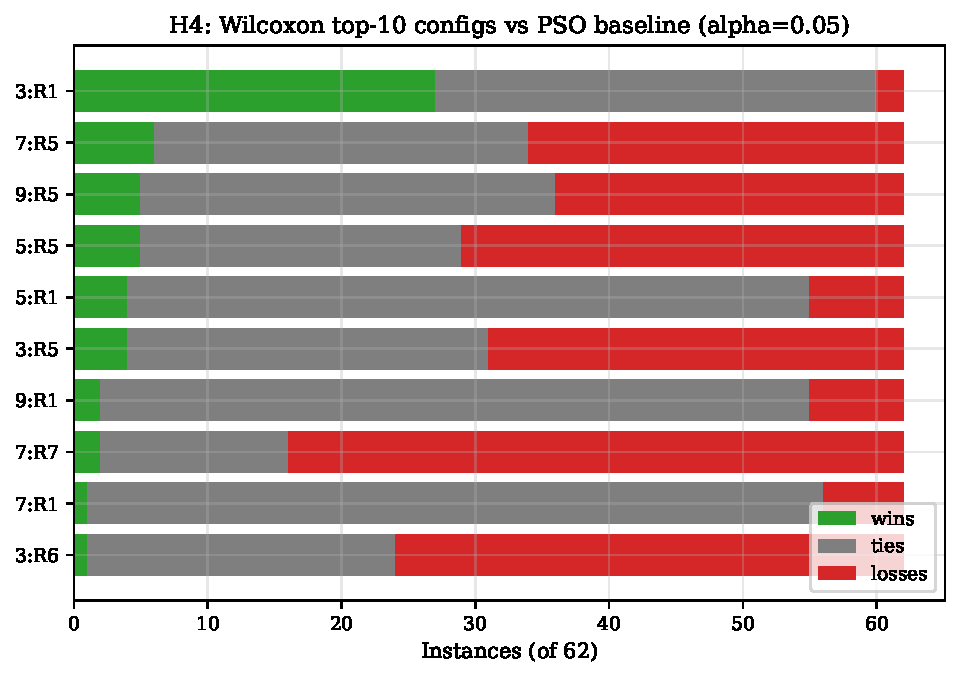
\includegraphics[width=0.85\linewidth]{figures/fig_h4_wilcoxon_bars.pdf}
%   \caption{TODO caption for fig_h4_wilcoxon_bars.}
%   \label{fig:fig_h4_wilcoxon_bars}
% \end{figure}
% \begin{figure}[h]
%   \centering
%   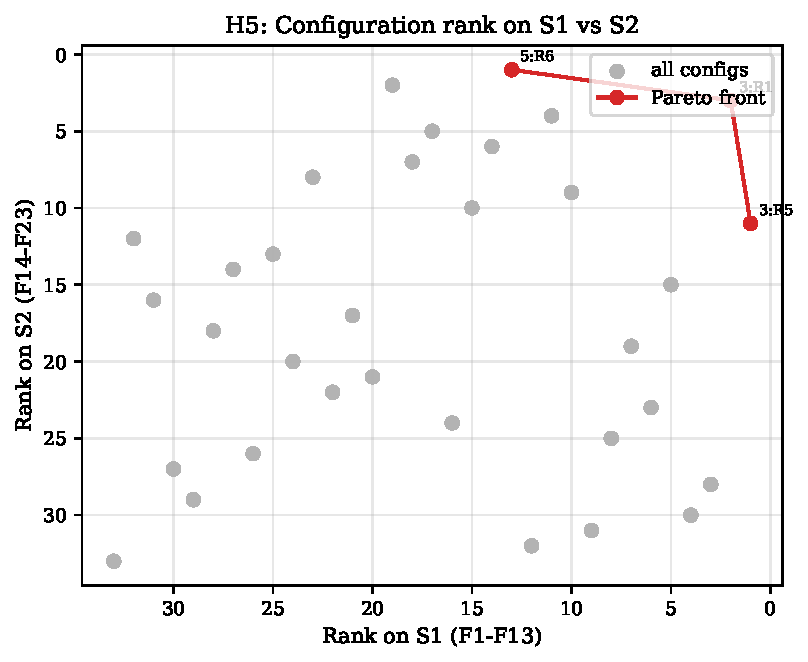
\includegraphics[width=0.85\linewidth]{figures/fig_pareto_s1_s2.pdf}
%   \caption{TODO caption for fig_pareto_s1_s2.}
%   \label{fig:fig_pareto_s1_s2}
% \end{figure}
% \begin{figure}[h]
%   \centering
%   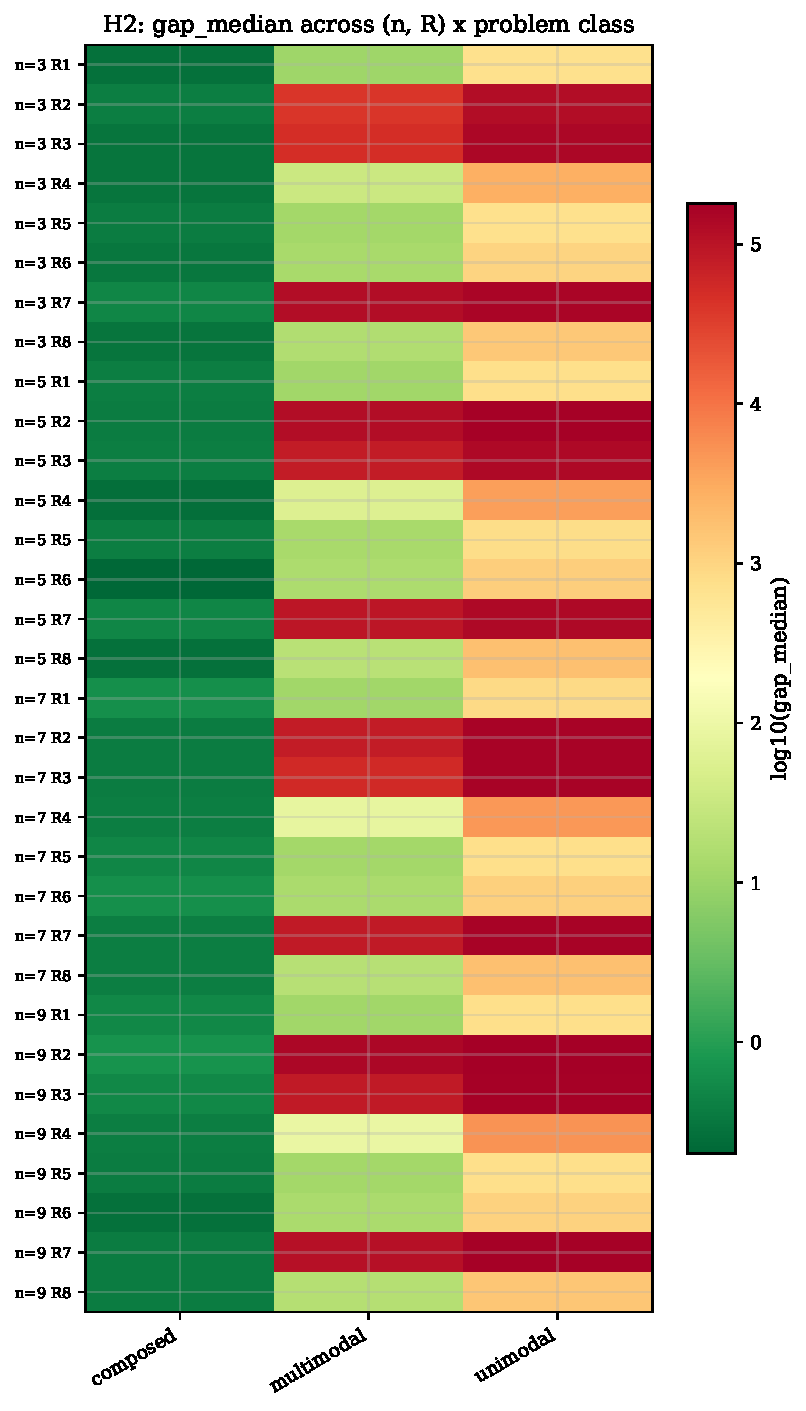
\includegraphics[width=0.85\linewidth]{figures/fig_rule_class_heatmap.pdf}
%   \caption{TODO caption for fig_rule_class_heatmap.}
%   \label{fig:fig_rule_class_heatmap}
% \end{figure}
% \begin{figure}[h]
%   \centering
%   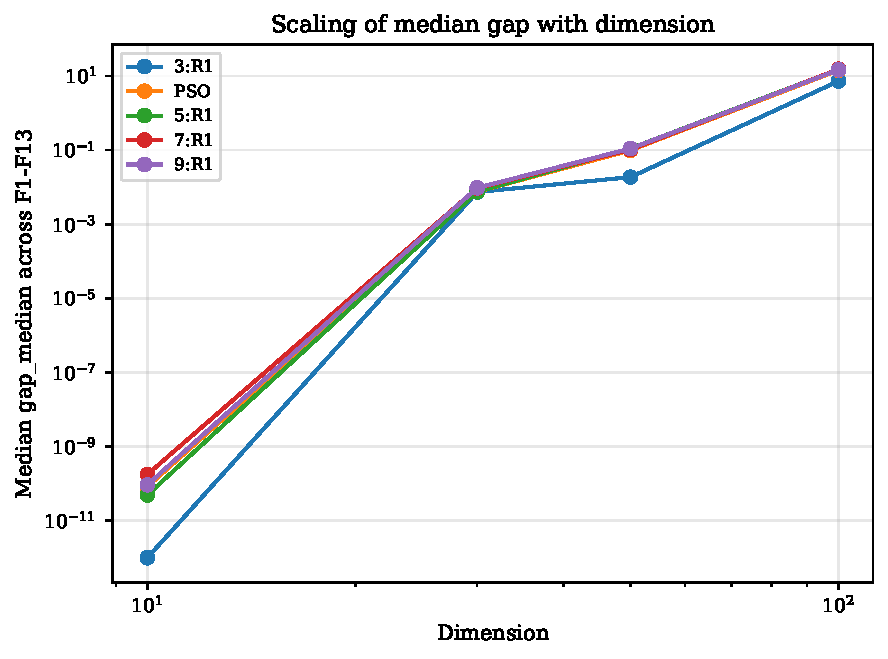
\includegraphics[width=0.85\linewidth]{figures/fig_scaling_curves.pdf}
%   \caption{TODO caption for fig_scaling_curves.}
%   \label{fig:fig_scaling_curves}
% \end{figure}
% \begin{figure}[h]
%   \centering
%   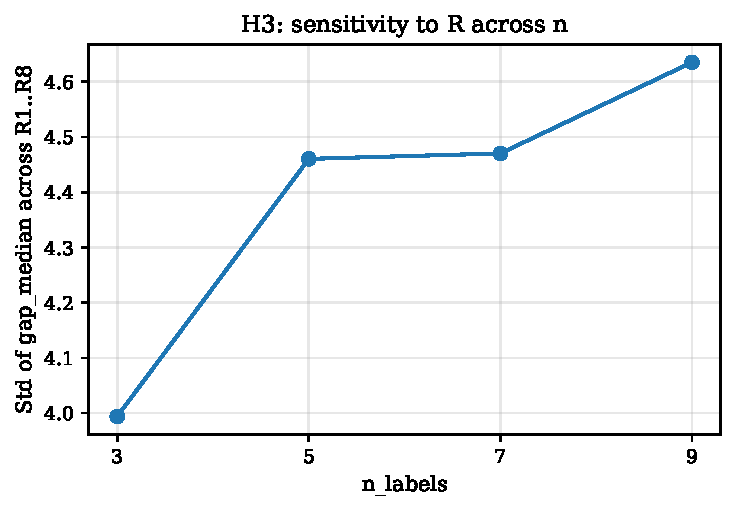
\includegraphics[width=0.85\linewidth]{figures/fig_std_R_vs_n.pdf}
%   \caption{TODO caption for fig_std_R_vs_n.}
%   \label{fig:fig_std_R_vs_n}
% \end{figure}

% ==== TABLES ====
% \begin{table}[h]
\centering
\caption{Wilcoxon signed-rank comparison of top-10 PSO\_FCS configurations against classical PSO (paired by run). Columns marked * apply Bonferroni correction over the full 32x62 grid.}
\label{tab:h4_wilcoxon}
\begin{tabular}{llllllllll}
\toprule
Config. & n & R & Wins & Ties & Losses & Wins* & Ties* & Losses* & A12 mean \\
\midrule
PSO\_FCS:O1:3:I1:R1 & 3.000 & R1 & 27 & 33 & 2 & 13 & 49 & 0 & 0.669 \\
PSO\_FCS:O1:7:I1:R5 & 7.000 & R5 & 6 & 28 & 28 & 1 & 43 & 18 & 0.363 \\
PSO\_FCS:O1:9:I1:R5 & 9.000 & R5 & 5 & 31 & 26 & 0 & 47 & 15 & 0.383 \\
PSO\_FCS:O1:5:I1:R5 & 5.000 & R5 & 5 & 24 & 33 & 0 & 38 & 24 & 0.304 \\
PSO\_FCS:O1:5:I1:R1 & 5.000 & R1 & 4 & 51 & 7 & 0 & 62 & 0 & 0.463 \\
PSO\_FCS:O1:3:I1:R5 & 3.000 & R5 & 4 & 27 & 31 & 0 & 48 & 14 & 0.358 \\
PSO\_FCS:O1:9:I1:R1 & 9.000 & R1 & 2 & 53 & 7 & 0 & 62 & 0 & 0.444 \\
PSO\_FCS:O1:7:I1:R7 & 7.000 & R7 & 2 & 14 & 46 & 0 & 23 & 39 & 0.173 \\
PSO\_FCS:O1:7:I1:R1 & 7.000 & R1 & 1 & 55 & 6 & 0 & 62 & 0 & 0.447 \\
PSO\_FCS:O1:3:I1:R6 & 3.000 & R6 & 1 & 23 & 38 & 0 & 35 & 27 & 0.225 \\
\bottomrule
\end{tabular}
\end{table}

% \begin{table}[h]
\centering
\caption{Summary of hypotheses H1--H5 with their governing statistic and verdict.}
\label{tab:hypothesis_summary}
\begin{tabular}{llll}
\toprule
Hypothesis & Statement & Key statistic & Verdict \\
\midrule
H1 & Granularity has diminishing returns & Friedman chi2 p=2.65e-200 & H0 rejected globally; within R1 the effect of n is \textless{} CD (not sig.) \\
H2 & Best R depends on problem class & tau(composed, unimodal)=0.08 & supported \\
H3 & Sensitivity to R decreases with n & n x R SRH p=0.34; peta\textasciicircum{}2(R)=0.063, peta\textasciicircum{}2(n)=0.0007 & rejected \\
H4 & PSO\_FCS beats PSO on \textgreater{}=50\% of instances & best config: 27 wins / 33 ties / 2 losses (of 62) & rejected under strict \textgreater{}=50\% criterion; supported = False \\
H5 & No static (n*, R*) dominates both S1 and S2 & tau(S1, S2)=0.09; argmin(S1)=PSO\_FCS:O1:3:I1:R5, argmin(S2)=PSO\_FCS:O1:5:I1:R6 & supported \\
\bottomrule
\end{tabular}
\end{table}

% \begin{table}[h]
\centering
\caption{Kendall's tau between rankings induced by the three problem classes (higher = more agreement).}
\label{tab:kendall_class}
\begin{tabular}{llll}
\toprule
class & composed & multimodal & unimodal \\
\midrule
composed & 1.000 & 0.080 & 0.083 \\
multimodal & 0.080 & 1.000 & 0.867 \\
unimodal & 0.083 & 0.867 & 1.000 \\
\bottomrule
\end{tabular}
\end{table}

% \begin{table}[h]
\centering
\caption{Log-log slope of median gap vs dimension for the five best- and five worst-scaling configurations.}
\label{tab:scaling_slopes}
\begin{tabular}{lllllll}
\toprule
Status & Config. & n & R & Mean slope & Median slope & Mean R\textasciicircum{}2 \\
\midrule
best-scaling & PSO\_FCS:O1:5:I1:R4 & 5.000 & R4 & 2.390 & 2.328 & 0.977 \\
best-scaling & PSO\_FCS:O1:9:I1:R4 & 9.000 & R4 & 2.238 & 2.385 & 0.985 \\
best-scaling & PSO\_FCS:O1:3:I1:R4 & 3.000 & R4 & 2.565 & 2.432 & 0.977 \\
best-scaling & PSO\_FCS:O1:7:I1:R4 & 7.000 & R4 & 2.348 & 2.435 & 0.982 \\
best-scaling & PSO\_FCS:O1:9:I1:R7 & 9.000 & R7 & 3.237 & 2.590 & 0.867 \\
worst-scaling & PSO\_FCS:O1:5:I1:R1 & 5.000 & R1 & 8.321 & 12.447 & 0.894 \\
worst-scaling & PSO\_FCS:O1:7:I1:R5 & 7.000 & R5 & 8.738 & 12.488 & 0.865 \\
worst-scaling & PSO\_FCS:O1:5:I1:R5 & 5.000 & R5 & 8.815 & 12.511 & 0.853 \\
worst-scaling & PSO\_FCS:O1:3:I1:R5 & 3.000 & R5 & 8.527 & 12.651 & 0.881 \\
worst-scaling & PSO\_FCS:O1:9:I1:R5 & 9.000 & R5 & 8.789 & 12.723 & 0.873 \\
\bottomrule
\end{tabular}
\end{table}

% \begin{table}[h]
\centering
\caption{Top 10 of the 33 configurations by mean Friedman rank over 62 benchmark instances (lower is better).}
\label{tab:top_configs}
\begin{tabular}{ll}
\toprule
Configuration & Mean rank \\
\midrule
FCS-3-R1 & 4.774 \\
PSO & 6.363 \\
FCS-5-R1 & 6.968 \\
FCS-7-R1 & 8.202 \\
FCS-9-R1 & 8.427 \\
FCS-9-R5 & 9.016 \\
FCS-3-R5 & 9.250 \\
FCS-7-R5 & 10.129 \\
FCS-3-R6 & 10.694 \\
FCS-5-R5 & 11.565 \\
\bottomrule
\end{tabular}
\end{table}



% ==== FIGURES ====
% \begin{figure}[h]
%   \centering
%   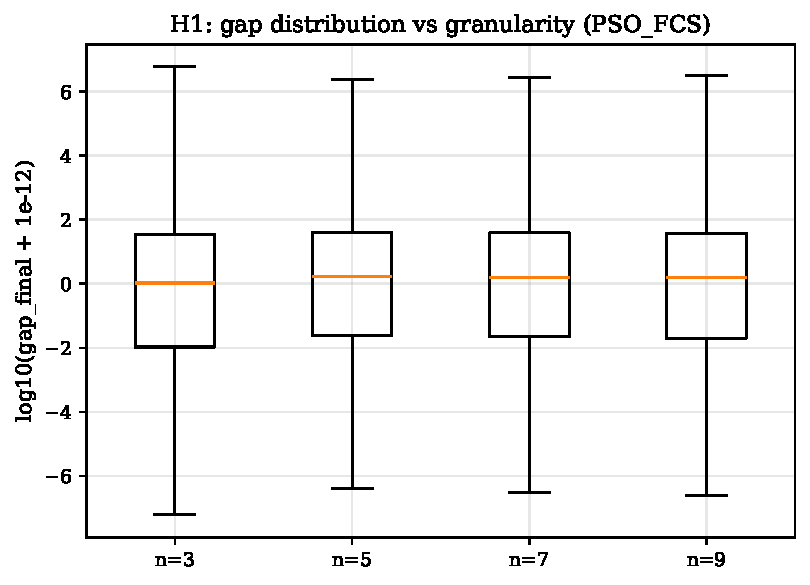
\includegraphics[width=0.85\linewidth]{figures/fig_boxplot_gap_by_n.pdf}
%   \caption{TODO caption for fig_boxplot_gap_by_n.}
%   \label{fig:fig_boxplot_gap_by_n}
% \end{figure}
% \begin{figure}[h]
%   \centering
%   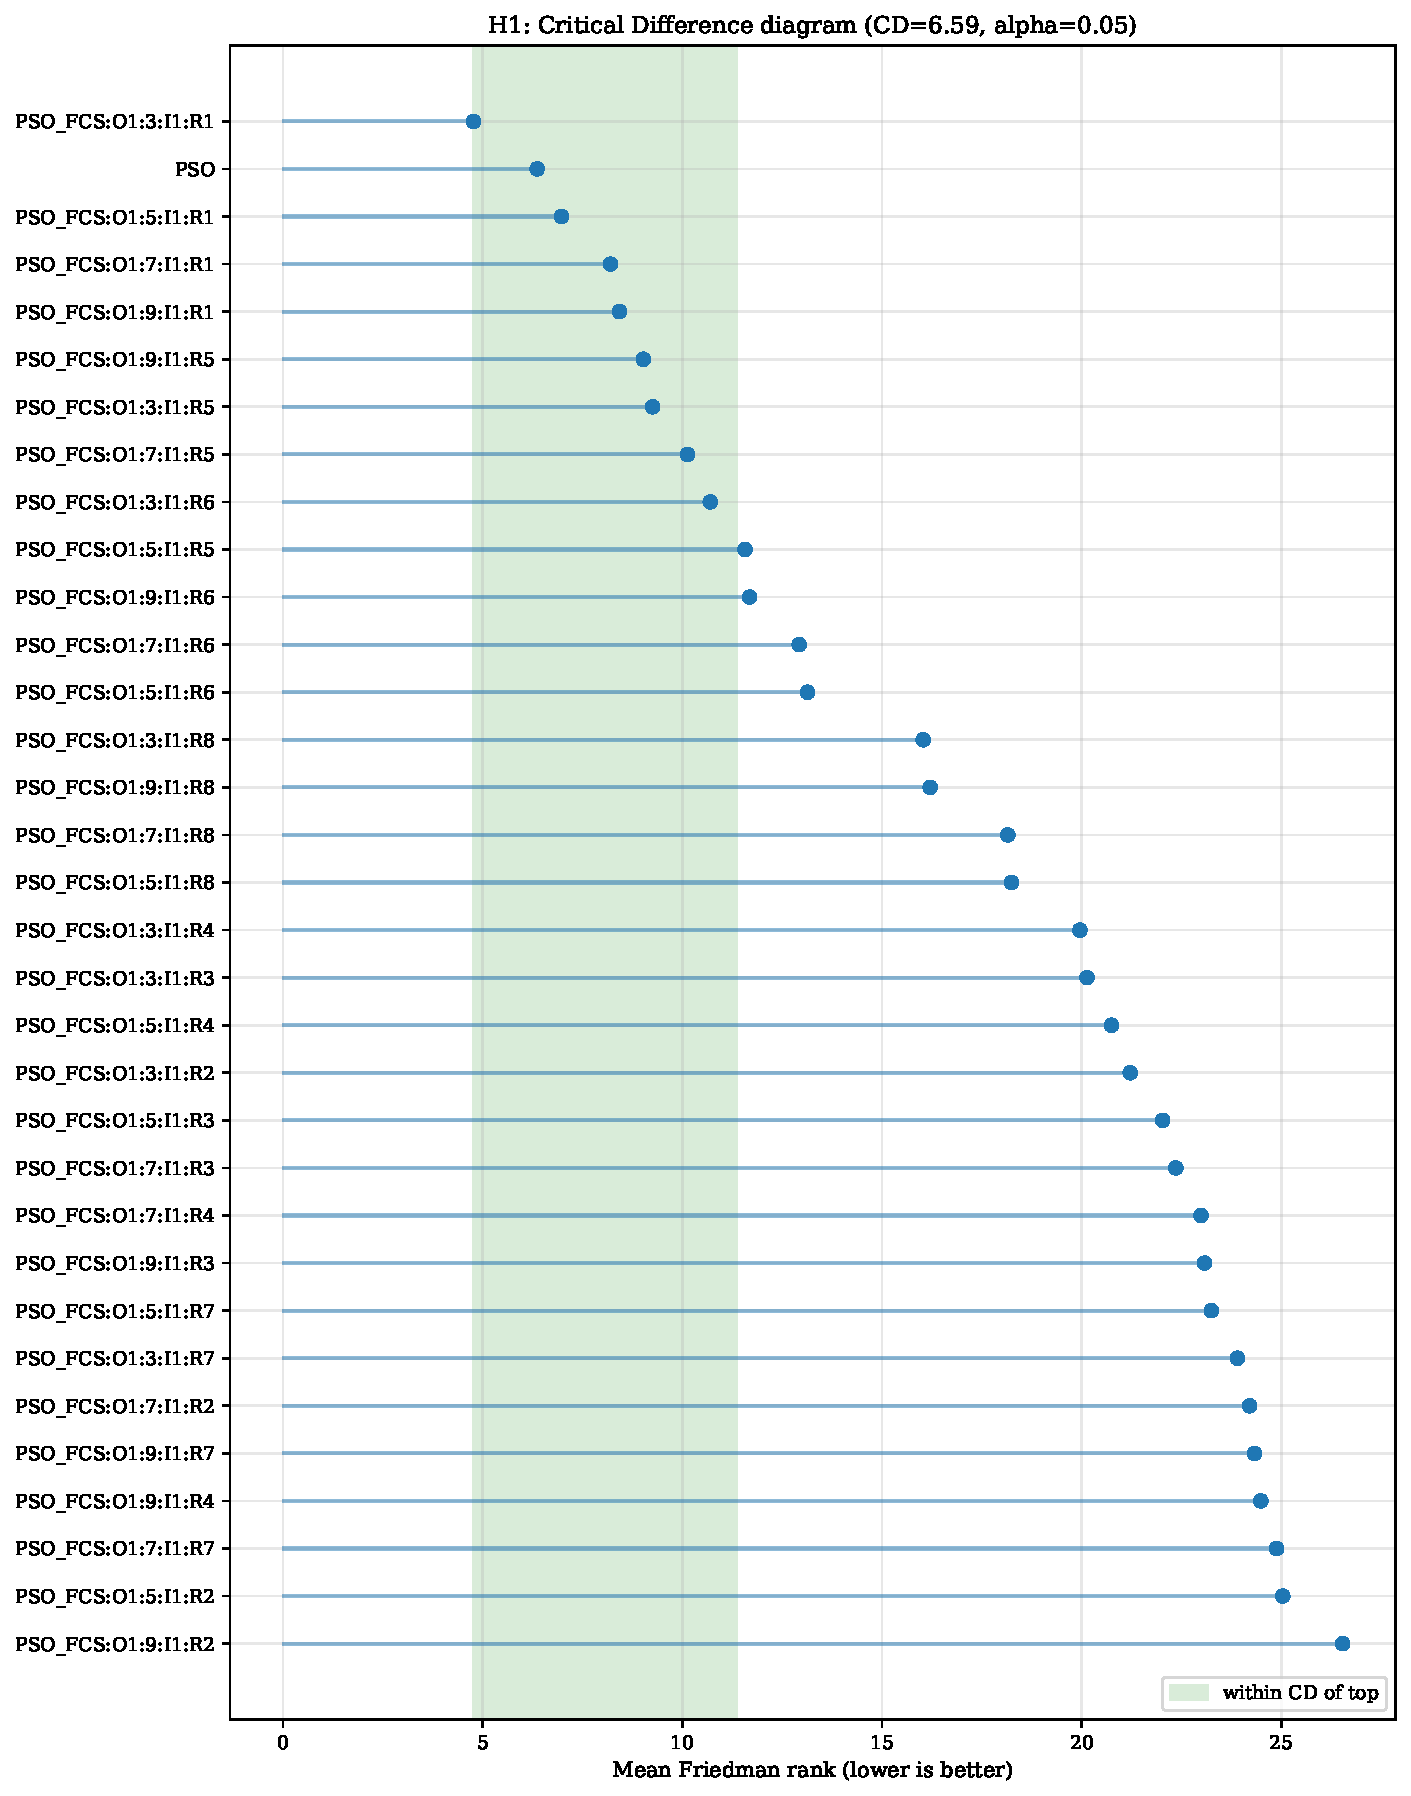
\includegraphics[width=0.85\linewidth]{figures/fig_cd_diagram_h1.pdf}
%   \caption{TODO caption for fig_cd_diagram_h1.}
%   \label{fig:fig_cd_diagram_h1}
% \end{figure}
% \begin{figure}[h]
%   \centering
%   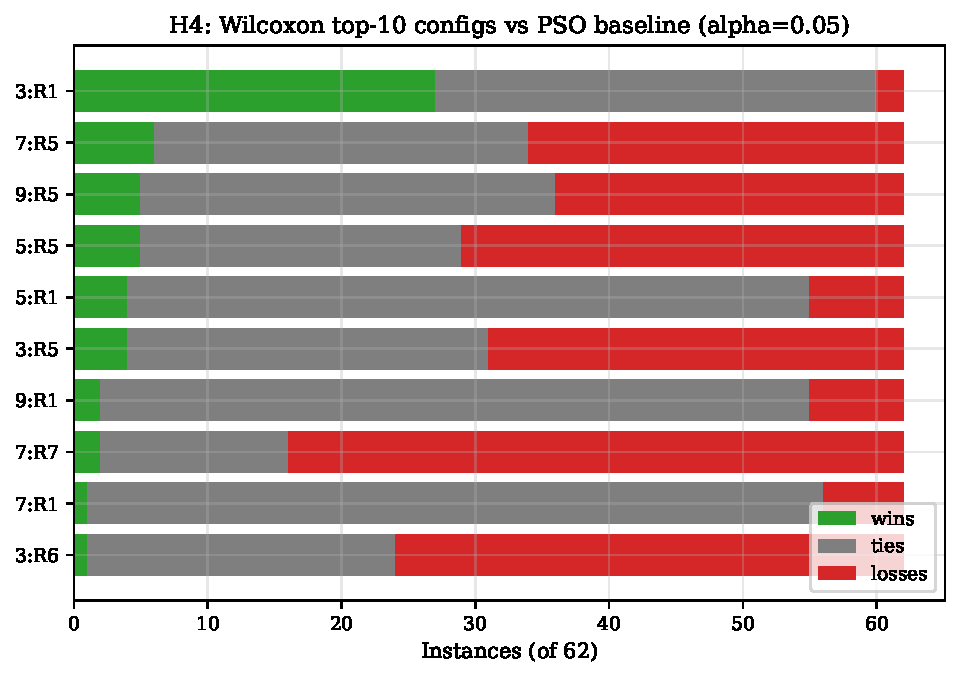
\includegraphics[width=0.85\linewidth]{figures/fig_h4_wilcoxon_bars.pdf}
%   \caption{TODO caption for fig_h4_wilcoxon_bars.}
%   \label{fig:fig_h4_wilcoxon_bars}
% \end{figure}
% \begin{figure}[h]
%   \centering
%   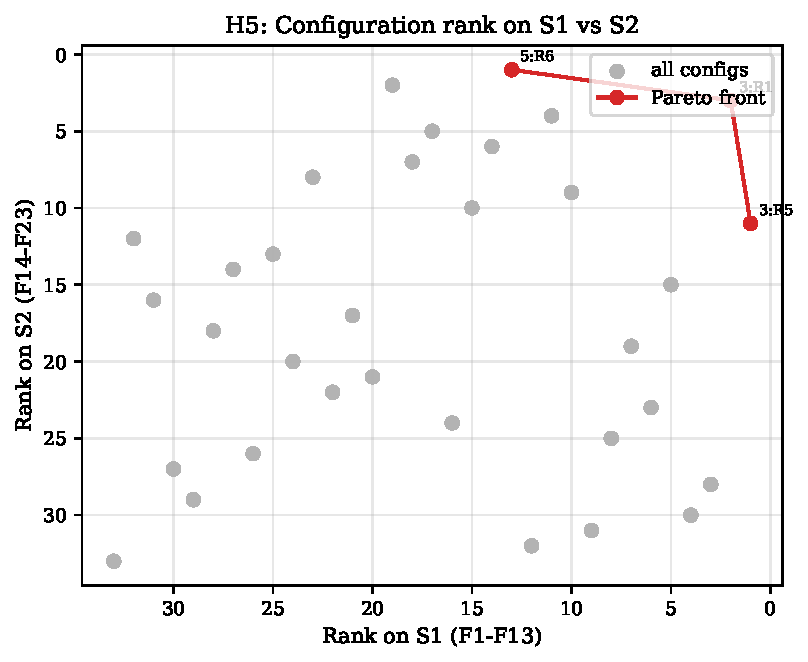
\includegraphics[width=0.85\linewidth]{figures/fig_pareto_s1_s2.pdf}
%   \caption{TODO caption for fig_pareto_s1_s2.}
%   \label{fig:fig_pareto_s1_s2}
% \end{figure}
% \begin{figure}[h]
%   \centering
%   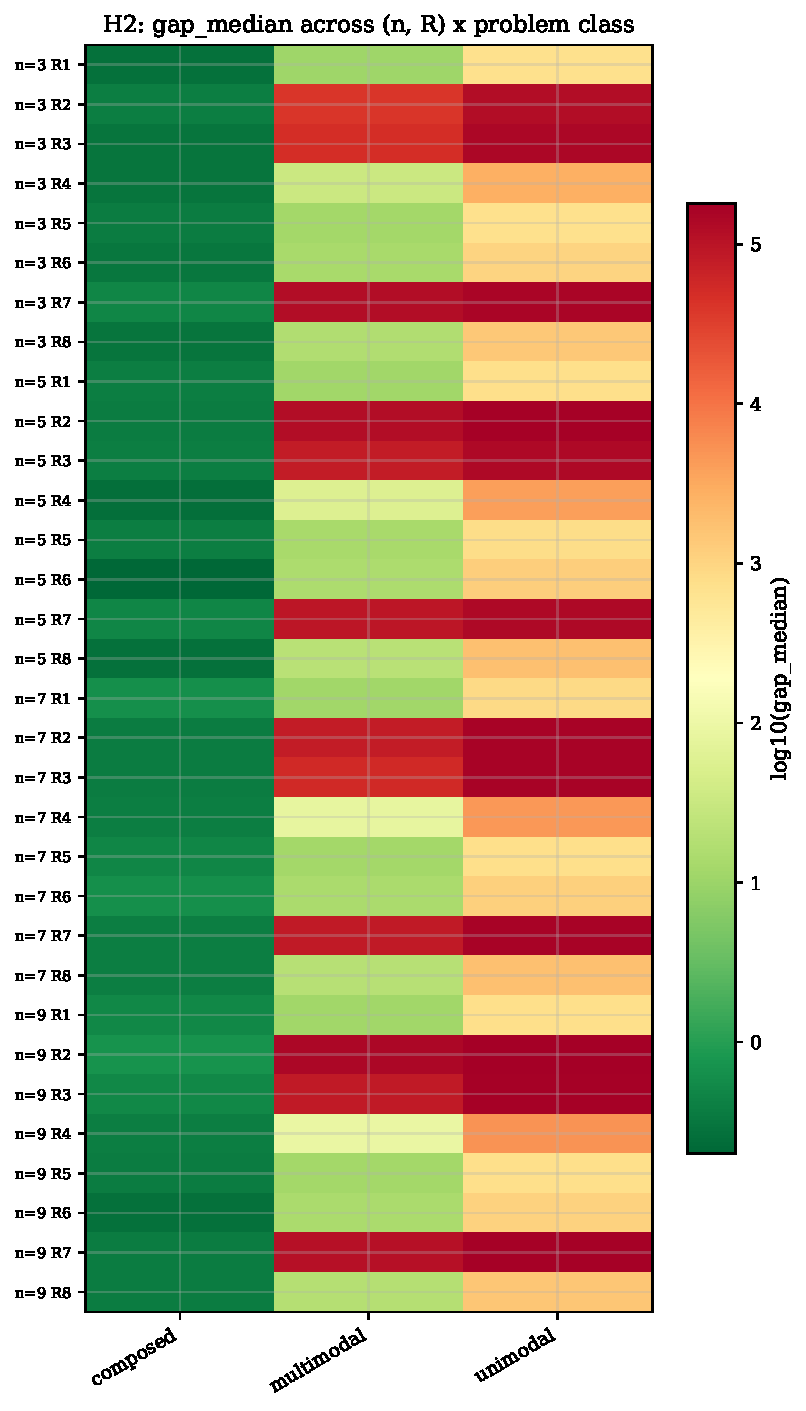
\includegraphics[width=0.85\linewidth]{figures/fig_rule_class_heatmap.pdf}
%   \caption{TODO caption for fig_rule_class_heatmap.}
%   \label{fig:fig_rule_class_heatmap}
% \end{figure}
% \begin{figure}[h]
%   \centering
%   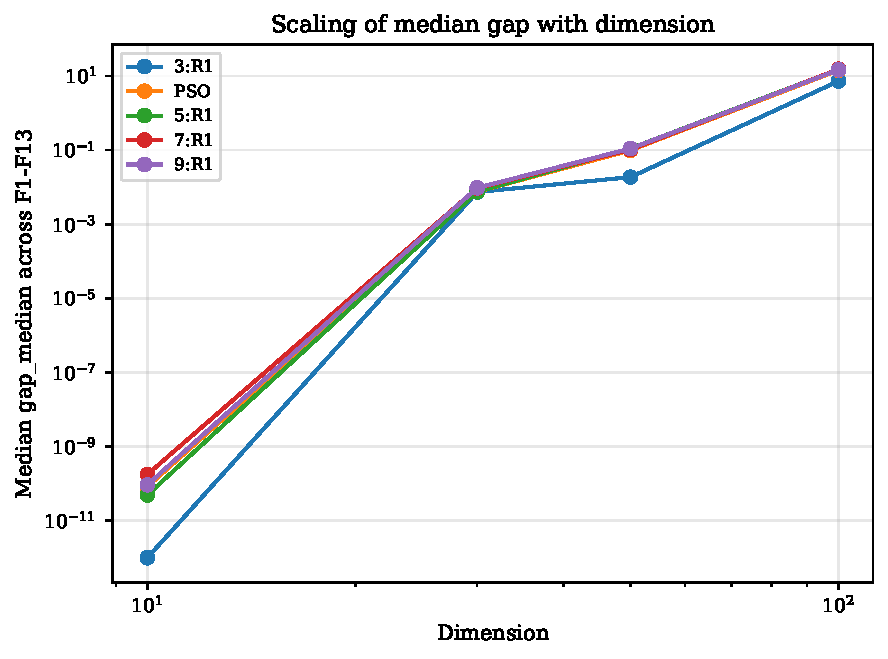
\includegraphics[width=0.85\linewidth]{figures/fig_scaling_curves.pdf}
%   \caption{TODO caption for fig_scaling_curves.}
%   \label{fig:fig_scaling_curves}
% \end{figure}
% \begin{figure}[h]
%   \centering
%   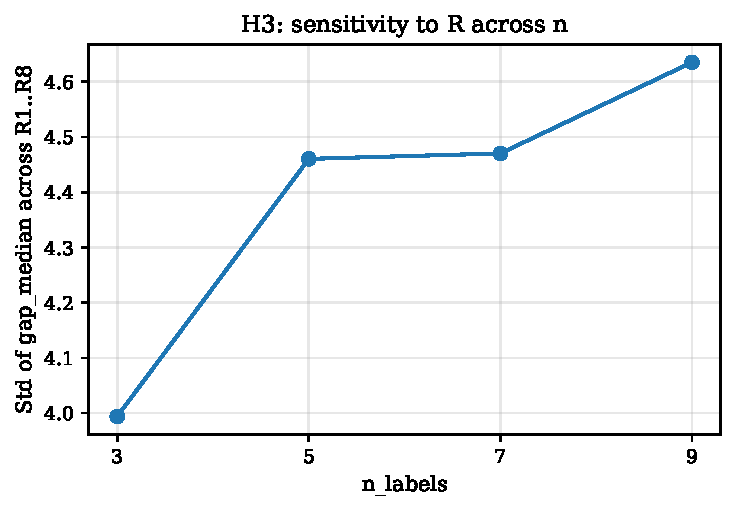
\includegraphics[width=0.85\linewidth]{figures/fig_std_R_vs_n.pdf}
%   \caption{TODO caption for fig_std_R_vs_n.}
%   \label{fig:fig_std_R_vs_n}
% \end{figure}

% ==== TABLES ====
% \begin{table}[h]
\centering
\caption{Wilcoxon signed-rank comparison of top-10 PSO\_FCS configurations against classical PSO (paired by run). Columns marked * apply Bonferroni correction over the full 32x62 grid.}
\label{tab:h4_wilcoxon}
\begin{tabular}{llllllllll}
\toprule
Config. & n & R & Wins & Ties & Losses & Wins* & Ties* & Losses* & A12 mean \\
\midrule
PSO\_FCS:O1:3:I1:R1 & 3.000 & R1 & 27 & 33 & 2 & 13 & 49 & 0 & 0.669 \\
PSO\_FCS:O1:7:I1:R5 & 7.000 & R5 & 6 & 28 & 28 & 1 & 43 & 18 & 0.363 \\
PSO\_FCS:O1:9:I1:R5 & 9.000 & R5 & 5 & 31 & 26 & 0 & 47 & 15 & 0.383 \\
PSO\_FCS:O1:5:I1:R5 & 5.000 & R5 & 5 & 24 & 33 & 0 & 38 & 24 & 0.304 \\
PSO\_FCS:O1:5:I1:R1 & 5.000 & R1 & 4 & 51 & 7 & 0 & 62 & 0 & 0.463 \\
PSO\_FCS:O1:3:I1:R5 & 3.000 & R5 & 4 & 27 & 31 & 0 & 48 & 14 & 0.358 \\
PSO\_FCS:O1:9:I1:R1 & 9.000 & R1 & 2 & 53 & 7 & 0 & 62 & 0 & 0.444 \\
PSO\_FCS:O1:7:I1:R7 & 7.000 & R7 & 2 & 14 & 46 & 0 & 23 & 39 & 0.173 \\
PSO\_FCS:O1:7:I1:R1 & 7.000 & R1 & 1 & 55 & 6 & 0 & 62 & 0 & 0.447 \\
PSO\_FCS:O1:3:I1:R6 & 3.000 & R6 & 1 & 23 & 38 & 0 & 35 & 27 & 0.225 \\
\bottomrule
\end{tabular}
\end{table}

% \begin{table}[h]
\centering
\caption{Summary of hypotheses H1--H5 with their governing statistic and verdict.}
\label{tab:hypothesis_summary}
\begin{tabular}{llll}
\toprule
Hypothesis & Statement & Key statistic & Verdict \\
\midrule
H1 & Granularity has diminishing returns & Friedman chi2 p=2.65e-200 & H0 rejected globally; within R1 the effect of n is \textless{} CD (not sig.) \\
H2 & Best R depends on problem class & tau(composed, unimodal)=0.08 & supported \\
H3 & Sensitivity to R decreases with n & n x R SRH p=0.34; peta\textasciicircum{}2(R)=0.063, peta\textasciicircum{}2(n)=0.0007 & rejected \\
H4 & PSO\_FCS beats PSO on \textgreater{}=50\% of instances & best config: 27 wins / 33 ties / 2 losses (of 62) & rejected under strict \textgreater{}=50\% criterion; supported = False \\
H5 & No static (n*, R*) dominates both S1 and S2 & tau(S1, S2)=0.09; argmin(S1)=PSO\_FCS:O1:3:I1:R5, argmin(S2)=PSO\_FCS:O1:5:I1:R6 & supported \\
\bottomrule
\end{tabular}
\end{table}

% \begin{table}[h]
\centering
\caption{Kendall's tau between rankings induced by the three problem classes (higher = more agreement).}
\label{tab:kendall_class}
\begin{tabular}{llll}
\toprule
class & composed & multimodal & unimodal \\
\midrule
composed & 1.000 & 0.080 & 0.083 \\
multimodal & 0.080 & 1.000 & 0.867 \\
unimodal & 0.083 & 0.867 & 1.000 \\
\bottomrule
\end{tabular}
\end{table}

% \begin{table}[h]
\centering
\caption{Log-log slope of median gap vs dimension for the five best- and five worst-scaling configurations.}
\label{tab:scaling_slopes}
\begin{tabular}{lllllll}
\toprule
Status & Config. & n & R & Mean slope & Median slope & Mean R\textasciicircum{}2 \\
\midrule
best-scaling & PSO\_FCS:O1:5:I1:R4 & 5.000 & R4 & 2.390 & 2.328 & 0.977 \\
best-scaling & PSO\_FCS:O1:9:I1:R4 & 9.000 & R4 & 2.238 & 2.385 & 0.985 \\
best-scaling & PSO\_FCS:O1:3:I1:R4 & 3.000 & R4 & 2.565 & 2.432 & 0.977 \\
best-scaling & PSO\_FCS:O1:7:I1:R4 & 7.000 & R4 & 2.348 & 2.435 & 0.982 \\
best-scaling & PSO\_FCS:O1:9:I1:R7 & 9.000 & R7 & 3.237 & 2.590 & 0.867 \\
worst-scaling & PSO\_FCS:O1:5:I1:R1 & 5.000 & R1 & 8.321 & 12.447 & 0.894 \\
worst-scaling & PSO\_FCS:O1:7:I1:R5 & 7.000 & R5 & 8.738 & 12.488 & 0.865 \\
worst-scaling & PSO\_FCS:O1:5:I1:R5 & 5.000 & R5 & 8.815 & 12.511 & 0.853 \\
worst-scaling & PSO\_FCS:O1:3:I1:R5 & 3.000 & R5 & 8.527 & 12.651 & 0.881 \\
worst-scaling & PSO\_FCS:O1:9:I1:R5 & 9.000 & R5 & 8.789 & 12.723 & 0.873 \\
\bottomrule
\end{tabular}
\end{table}

% \begin{table}[h]
\centering
\caption{Top 10 of the 33 configurations by mean Friedman rank over 62 benchmark instances (lower is better).}
\label{tab:top_configs}
\begin{tabular}{ll}
\toprule
Configuration & Mean rank \\
\midrule
FCS-3-R1 & 4.774 \\
PSO & 6.363 \\
FCS-5-R1 & 6.968 \\
FCS-7-R1 & 8.202 \\
FCS-9-R1 & 8.427 \\
FCS-9-R5 & 9.016 \\
FCS-3-R5 & 9.250 \\
FCS-7-R5 & 10.129 \\
FCS-3-R6 & 10.694 \\
FCS-5-R5 & 11.565 \\
\bottomrule
\end{tabular}
\end{table}



% ==== FIGURES ====
% \begin{figure}[h]
%   \centering
%   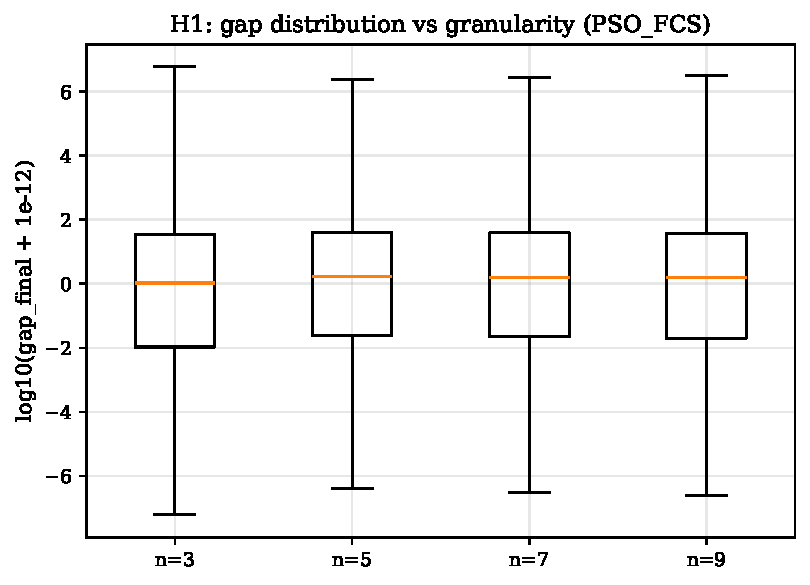
\includegraphics[width=0.85\linewidth]{figures/fig_boxplot_gap_by_n.pdf}
%   \caption{TODO caption for fig_boxplot_gap_by_n.}
%   \label{fig:fig_boxplot_gap_by_n}
% \end{figure}
% \begin{figure}[h]
%   \centering
%   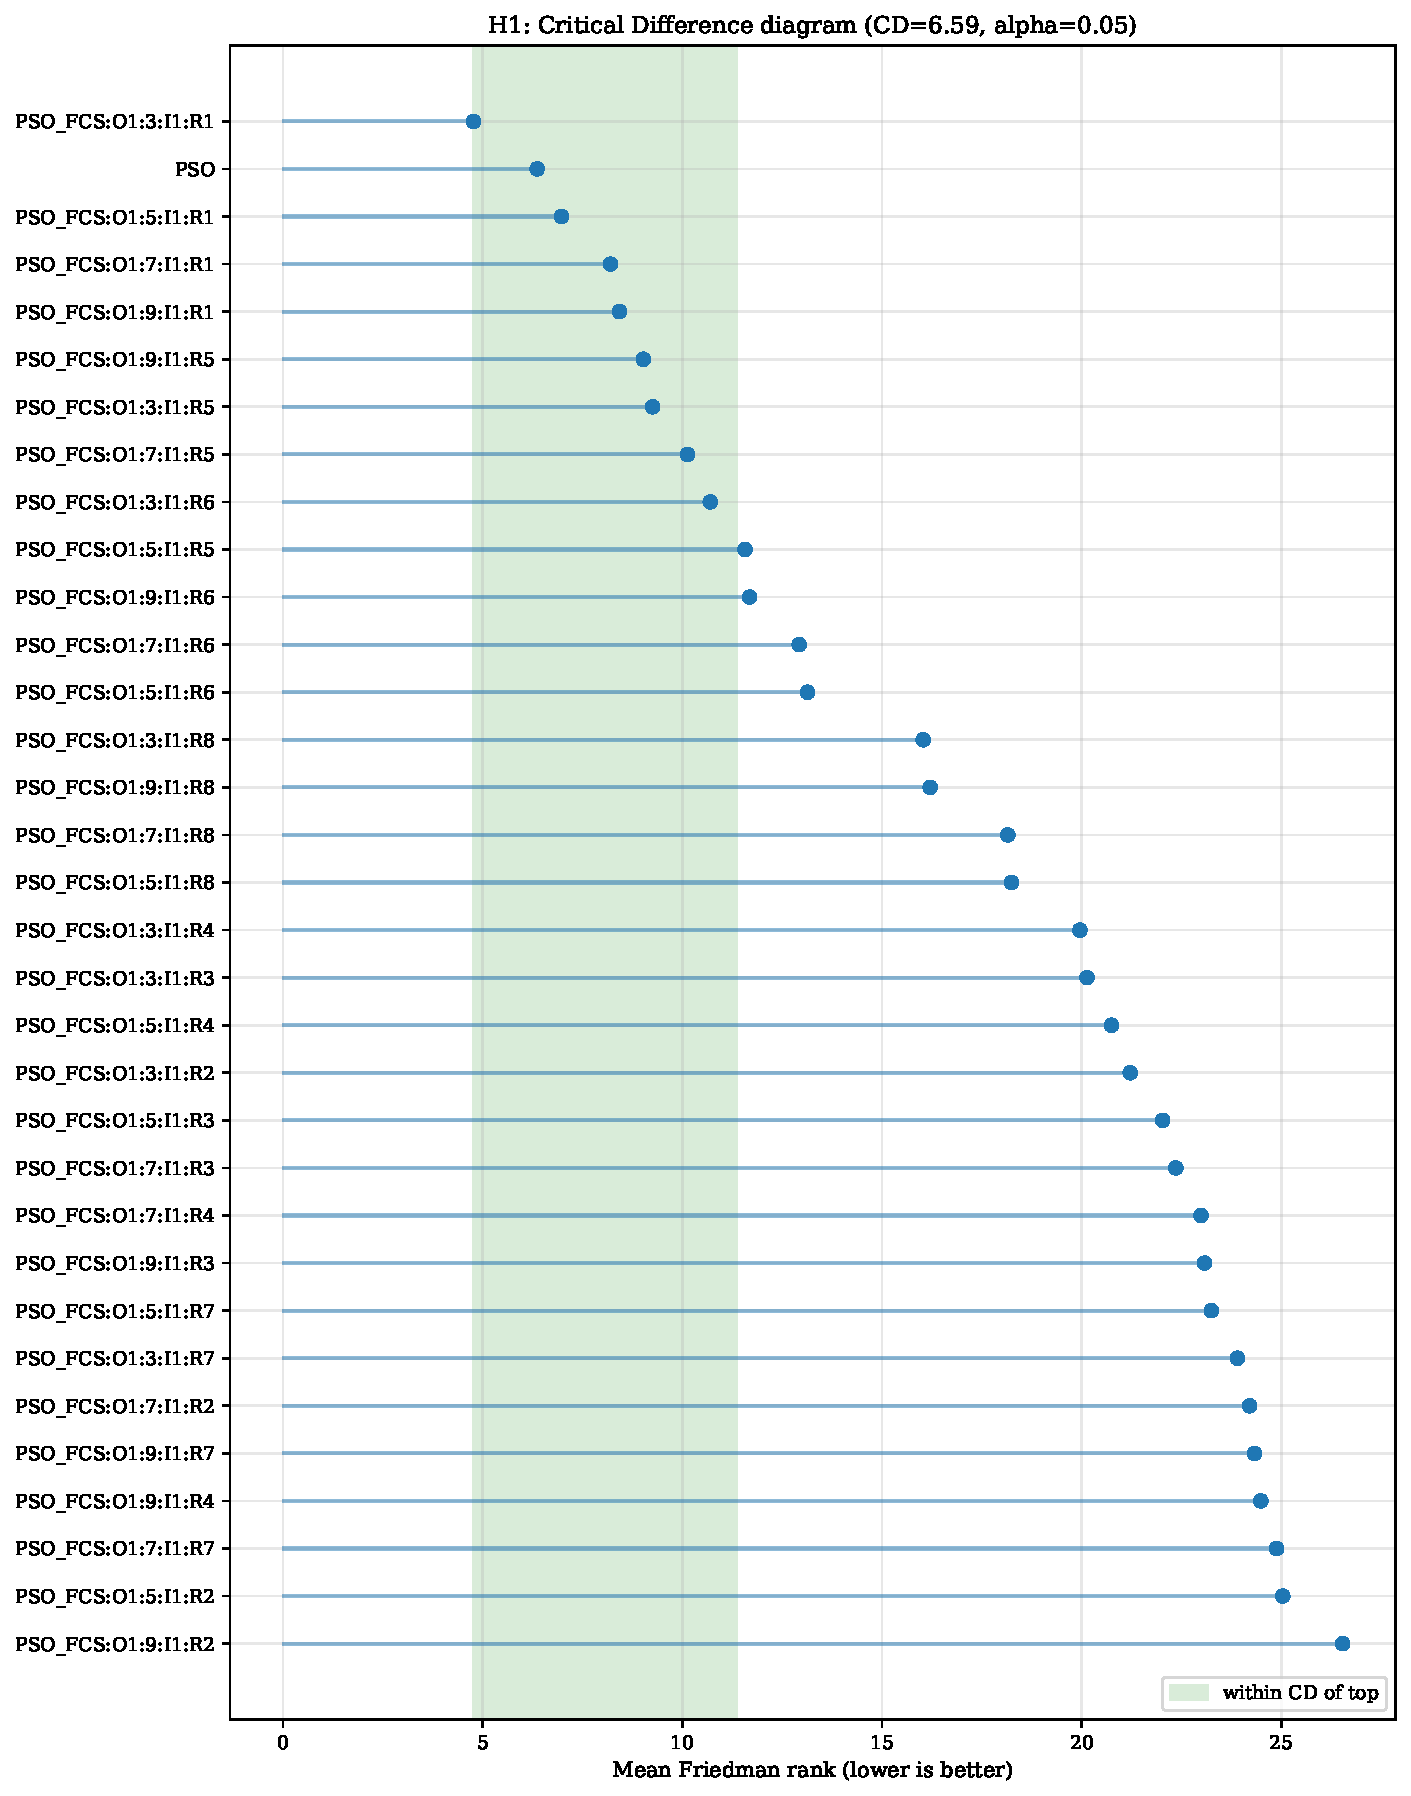
\includegraphics[width=0.85\linewidth]{figures/fig_cd_diagram_h1.pdf}
%   \caption{TODO caption for fig_cd_diagram_h1.}
%   \label{fig:fig_cd_diagram_h1}
% \end{figure}
% \begin{figure}[h]
%   \centering
%   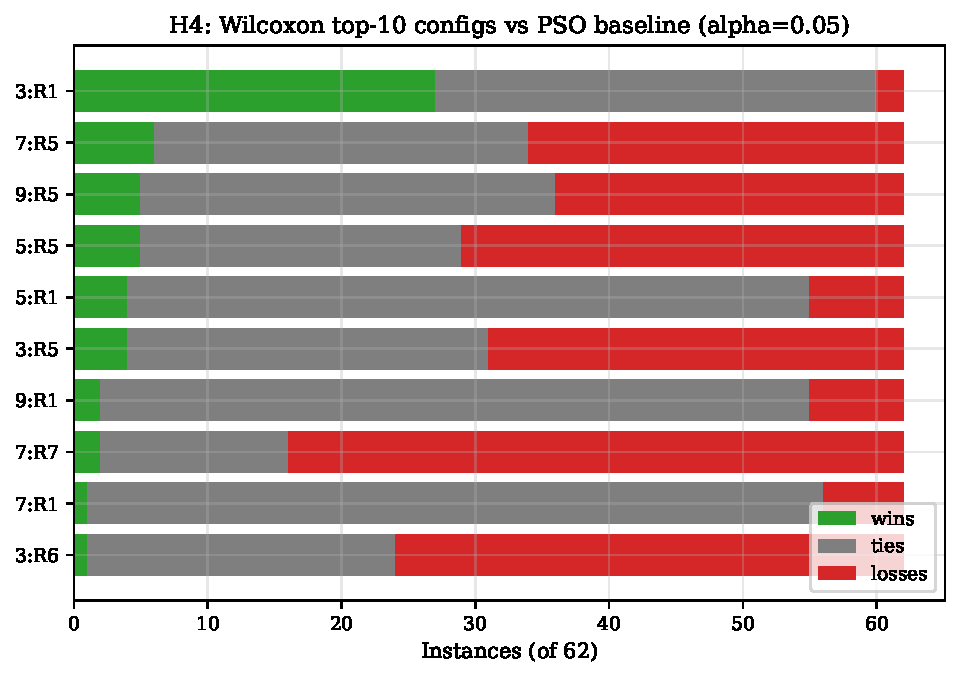
\includegraphics[width=0.85\linewidth]{figures/fig_h4_wilcoxon_bars.pdf}
%   \caption{TODO caption for fig_h4_wilcoxon_bars.}
%   \label{fig:fig_h4_wilcoxon_bars}
% \end{figure}
% \begin{figure}[h]
%   \centering
%   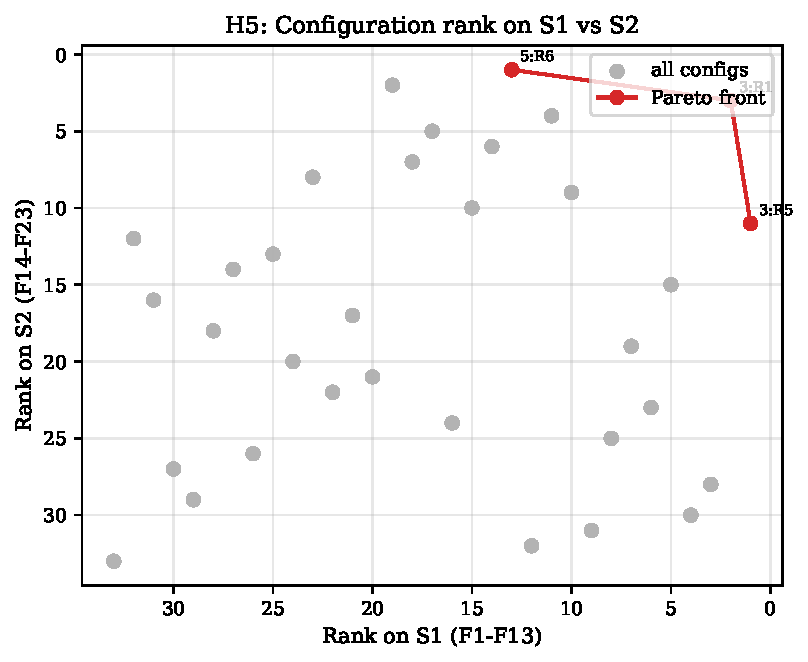
\includegraphics[width=0.85\linewidth]{figures/fig_pareto_s1_s2.pdf}
%   \caption{TODO caption for fig_pareto_s1_s2.}
%   \label{fig:fig_pareto_s1_s2}
% \end{figure}
% \begin{figure}[h]
%   \centering
%   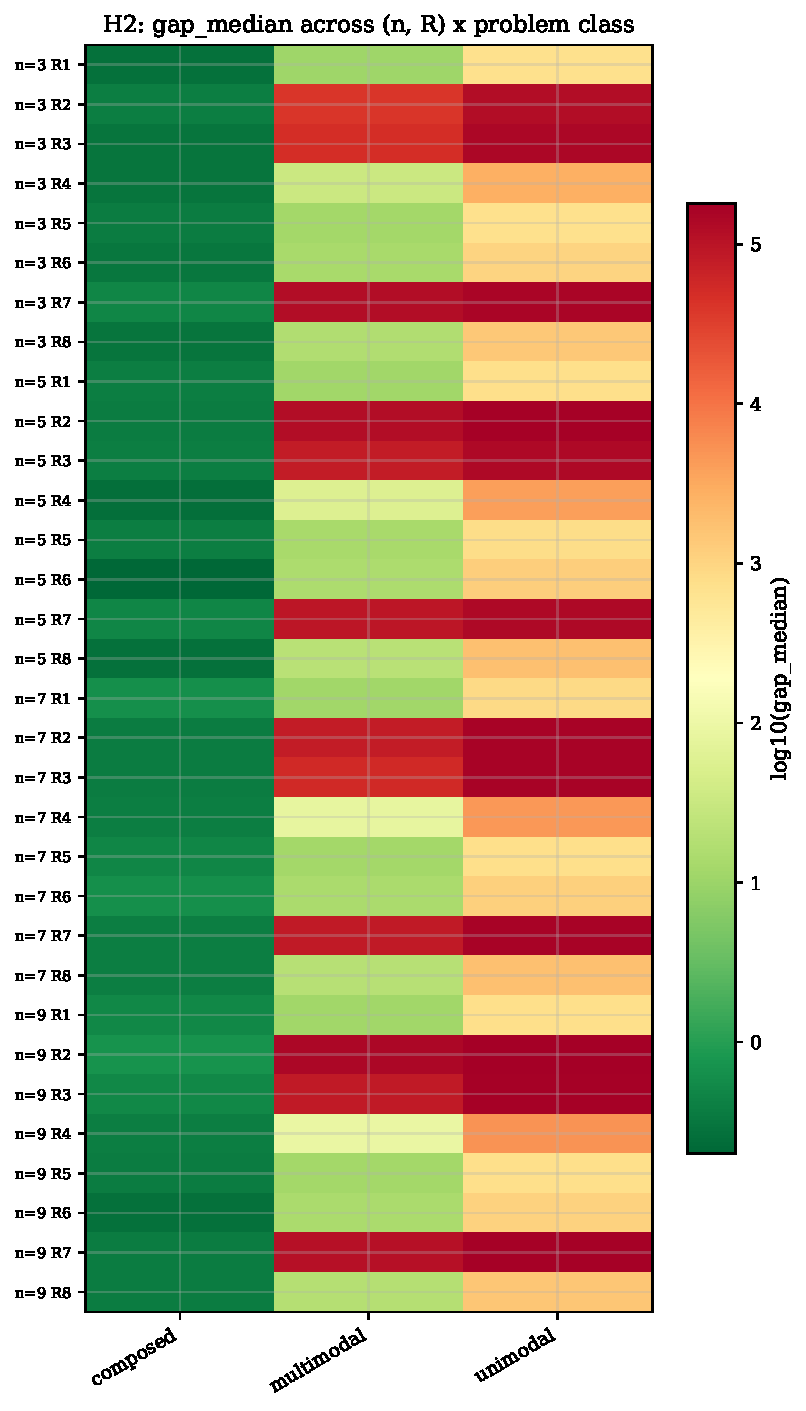
\includegraphics[width=0.85\linewidth]{figures/fig_rule_class_heatmap.pdf}
%   \caption{TODO caption for fig_rule_class_heatmap.}
%   \label{fig:fig_rule_class_heatmap}
% \end{figure}
% \begin{figure}[h]
%   \centering
%   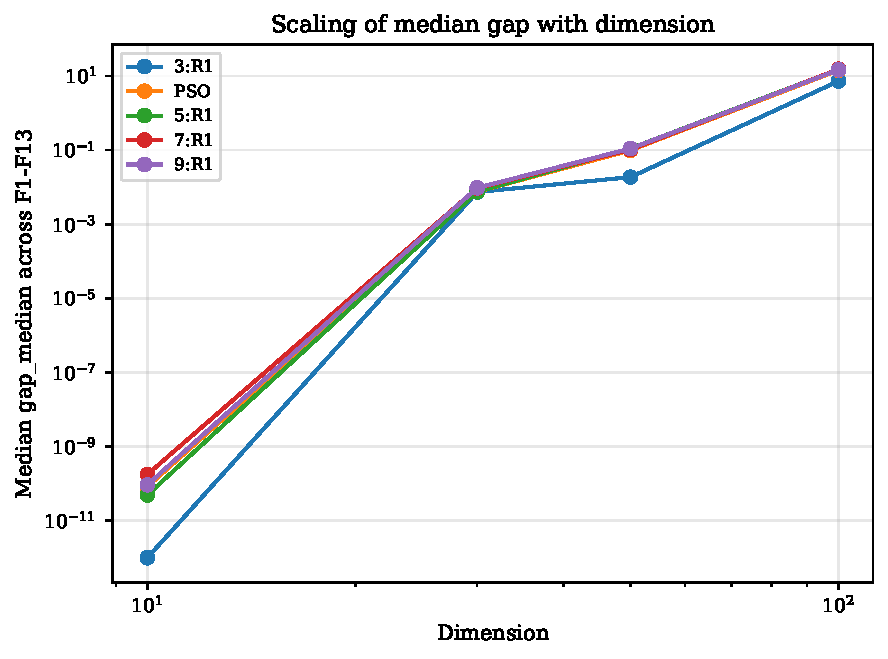
\includegraphics[width=0.85\linewidth]{figures/fig_scaling_curves.pdf}
%   \caption{TODO caption for fig_scaling_curves.}
%   \label{fig:fig_scaling_curves}
% \end{figure}
% \begin{figure}[h]
%   \centering
%   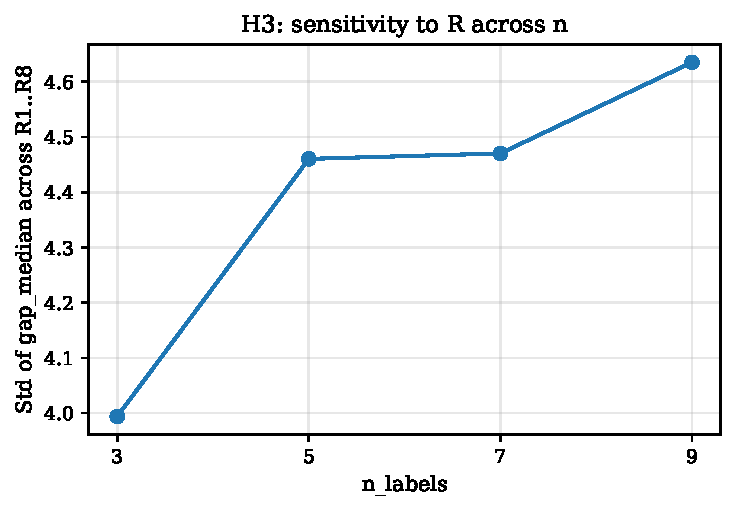
\includegraphics[width=0.85\linewidth]{figures/fig_std_R_vs_n.pdf}
%   \caption{TODO caption for fig_std_R_vs_n.}
%   \label{fig:fig_std_R_vs_n}
% \end{figure}

% ==== TABLES ====
% \begin{table}[h]
\centering
\caption{Wilcoxon signed-rank comparison of top-10 PSO\_FCS configurations against classical PSO (paired by run). Columns marked * apply Bonferroni correction over the full 32x62 grid.}
\label{tab:h4_wilcoxon}
\begin{tabular}{llllllllll}
\toprule
Config. & n & R & Wins & Ties & Losses & Wins* & Ties* & Losses* & A12 mean \\
\midrule
PSO\_FCS:O1:3:I1:R1 & 3.000 & R1 & 27 & 33 & 2 & 13 & 49 & 0 & 0.669 \\
PSO\_FCS:O1:7:I1:R5 & 7.000 & R5 & 6 & 28 & 28 & 1 & 43 & 18 & 0.363 \\
PSO\_FCS:O1:9:I1:R5 & 9.000 & R5 & 5 & 31 & 26 & 0 & 47 & 15 & 0.383 \\
PSO\_FCS:O1:5:I1:R5 & 5.000 & R5 & 5 & 24 & 33 & 0 & 38 & 24 & 0.304 \\
PSO\_FCS:O1:5:I1:R1 & 5.000 & R1 & 4 & 51 & 7 & 0 & 62 & 0 & 0.463 \\
PSO\_FCS:O1:3:I1:R5 & 3.000 & R5 & 4 & 27 & 31 & 0 & 48 & 14 & 0.358 \\
PSO\_FCS:O1:9:I1:R1 & 9.000 & R1 & 2 & 53 & 7 & 0 & 62 & 0 & 0.444 \\
PSO\_FCS:O1:7:I1:R7 & 7.000 & R7 & 2 & 14 & 46 & 0 & 23 & 39 & 0.173 \\
PSO\_FCS:O1:7:I1:R1 & 7.000 & R1 & 1 & 55 & 6 & 0 & 62 & 0 & 0.447 \\
PSO\_FCS:O1:3:I1:R6 & 3.000 & R6 & 1 & 23 & 38 & 0 & 35 & 27 & 0.225 \\
\bottomrule
\end{tabular}
\end{table}

% \begin{table}[h]
\centering
\caption{Summary of hypotheses H1--H5 with their governing statistic and verdict.}
\label{tab:hypothesis_summary}
\begin{tabular}{llll}
\toprule
Hypothesis & Statement & Key statistic & Verdict \\
\midrule
H1 & Granularity has diminishing returns & Friedman chi2 p=2.65e-200 & H0 rejected globally; within R1 the effect of n is \textless{} CD (not sig.) \\
H2 & Best R depends on problem class & tau(composed, unimodal)=0.08 & supported \\
H3 & Sensitivity to R decreases with n & n x R SRH p=0.34; peta\textasciicircum{}2(R)=0.063, peta\textasciicircum{}2(n)=0.0007 & rejected \\
H4 & PSO\_FCS beats PSO on \textgreater{}=50\% of instances & best config: 27 wins / 33 ties / 2 losses (of 62) & rejected under strict \textgreater{}=50\% criterion; supported = False \\
H5 & No static (n*, R*) dominates both S1 and S2 & tau(S1, S2)=0.09; argmin(S1)=PSO\_FCS:O1:3:I1:R5, argmin(S2)=PSO\_FCS:O1:5:I1:R6 & supported \\
\bottomrule
\end{tabular}
\end{table}

% \begin{table}[h]
\centering
\caption{Kendall's tau between rankings induced by the three problem classes (higher = more agreement).}
\label{tab:kendall_class}
\begin{tabular}{llll}
\toprule
class & composed & multimodal & unimodal \\
\midrule
composed & 1.000 & 0.080 & 0.083 \\
multimodal & 0.080 & 1.000 & 0.867 \\
unimodal & 0.083 & 0.867 & 1.000 \\
\bottomrule
\end{tabular}
\end{table}

% \begin{table}[h]
\centering
\caption{Log-log slope of median gap vs dimension for the five best- and five worst-scaling configurations.}
\label{tab:scaling_slopes}
\begin{tabular}{lllllll}
\toprule
Status & Config. & n & R & Mean slope & Median slope & Mean R\textasciicircum{}2 \\
\midrule
best-scaling & PSO\_FCS:O1:5:I1:R4 & 5.000 & R4 & 2.390 & 2.328 & 0.977 \\
best-scaling & PSO\_FCS:O1:9:I1:R4 & 9.000 & R4 & 2.238 & 2.385 & 0.985 \\
best-scaling & PSO\_FCS:O1:3:I1:R4 & 3.000 & R4 & 2.565 & 2.432 & 0.977 \\
best-scaling & PSO\_FCS:O1:7:I1:R4 & 7.000 & R4 & 2.348 & 2.435 & 0.982 \\
best-scaling & PSO\_FCS:O1:9:I1:R7 & 9.000 & R7 & 3.237 & 2.590 & 0.867 \\
worst-scaling & PSO\_FCS:O1:5:I1:R1 & 5.000 & R1 & 8.321 & 12.447 & 0.894 \\
worst-scaling & PSO\_FCS:O1:7:I1:R5 & 7.000 & R5 & 8.738 & 12.488 & 0.865 \\
worst-scaling & PSO\_FCS:O1:5:I1:R5 & 5.000 & R5 & 8.815 & 12.511 & 0.853 \\
worst-scaling & PSO\_FCS:O1:3:I1:R5 & 3.000 & R5 & 8.527 & 12.651 & 0.881 \\
worst-scaling & PSO\_FCS:O1:9:I1:R5 & 9.000 & R5 & 8.789 & 12.723 & 0.873 \\
\bottomrule
\end{tabular}
\end{table}

% \begin{table}[h]
\centering
\caption{Top 10 of the 33 configurations by mean Friedman rank over 62 benchmark instances (lower is better).}
\label{tab:top_configs}
\begin{tabular}{ll}
\toprule
Configuration & Mean rank \\
\midrule
FCS-3-R1 & 4.774 \\
PSO & 6.363 \\
FCS-5-R1 & 6.968 \\
FCS-7-R1 & 8.202 \\
FCS-9-R1 & 8.427 \\
FCS-9-R5 & 9.016 \\
FCS-3-R5 & 9.250 \\
FCS-7-R5 & 10.129 \\
FCS-3-R6 & 10.694 \\
FCS-5-R5 & 11.565 \\
\bottomrule
\end{tabular}
\end{table}

